\chapter[Assessment of freezing of gait]{Assessment of freezing of gait}
\label{ch6}

\section{State of knowledge}
\label{ch6_1}

Freezing of gait (FOG) is a~frequent disabling symptom in patients with PD that is characterized by sudden and transient interruptions to walking, which according to the literature, tends to occur when initiating walking, turning, or facing an obstacle or narrow path~\cite{Nutt2011}. As reported by the previous studies, FOG has been diagnosed in approximately half of the patients with PD and is more likely to occur in advanced stages of the disease~\cite{Bartels2003}. As reported by several studies \cite{Giladi1997, Giladi2001, Macht2007}, patients suffering from FOG experience problems in controlling and modulating their gait, especially during its initiation and changes in direction or speed. Gait disorders associated with FOG in PD \cite{Giladi1997, Giladi2001, Morris2001b} can lead to poor locomotion, postural instability, and eventually to serious fall-related injuries \cite{Gray2000, Schaafsma2003} reducing the quality of life of the patients. Despite the fact that FOG is a~very problematic aspect occurring in most patients with PD~\cite{Giladi2001c}, the exact pathophysiological mechanism underlying FOG in PD remains unexplained \cite{Shine2011, Vesely2016, Virmani2015}.

In $2001$, Giladi et al.~\cite{Giladi2001b} studied development of freezing of gait in patients with idiopathic PD. Based on the analysis of data from $800$ patients with early PD from the Deprenyl and Tocopherol Antioxidative Therapy of Parkinsonism (DATATOP) clinical trial, they reported a~strong association between FOG and speech abnormalities, both assessed by the Unified Parkinson's Disease Rating Scale (UPDRS), part~III, evaluation of motor function~\cite{Fahn1987}. However, due to the very limited ability of item $18$ of this particular clinical rating scale to sufficiently describe a~variety of voice/speech disorders occurring with HD, the authors simply concluded that there might be some common pathophysiological mechanisms between FOG and HD that should be investigated in future research.

In $2003$, Bartels et al.~\cite{Bartels2003} studied a~relationship between FOG (quantified by FOG frequency based on the assessment of $3$ independent viewers who watched videotapes and rated a~performance of a~$130$\,m walk) and other clinical features of PD (again evaluated by UPDRS, including speech) in $19$ PD patients who were assessed in their OFF (prior to levodopa dosage use) and ON (after the levodopa dosage use) state. They reported that the FOG frequency was not correlated with other parkinsonian manifestations in the OFF state, and it was related to speech and writing only in the ON state. The authors concluded that FOG is an independent motor symptom, caused by a~paroxysmal pathology that is different from that responsible for bradykinesia, rigidity or postural instability in PD.

In $2005$, A. M. Goberman~\cite{Goberman2005b} published a~study dealing with the correlation analysis between $16$ acoustic measures (quantifying multidimensional HD in the area of phonation, articulation, and prosody) and non-speech motor performance (once again assessed by UPDRS) in $9$ patients with idiopathic PD. After the analysis, $3$ significant and positive correlations were identified between gait deficits and these acoustic parameters: the standard deviation of fundamental frequency, percent pause time calculated from monologue, and finally percent pause time calculated from a~reading task. Based on the observation that some acoustic measures were found correlated with both axial motor symptoms (e.\,g., gait, facial expression) and non-axial motor symptoms (e.\,g. resting tremor, bradykinesia), the author also concluded that some voice/speech deficits in PD may result from dopaminergic lesions, while others are likely to result from non-dopaminergic ones.

In $2007$, Moreau et al.~\cite{Moreau2007} were interested in the relationship between oral festination (quantified by acoustic parameters based on diadochokinetic rate), and gait festination and FOG separately. With this approach, the authors analysed the tendency of PD patients to speed up when performing repetitive movements. They enrolled $40$ PD patients ($17$ presented both gait festination and FOG, $5$ presented gait festination alone, $9$ presented FOG alone, and $9$ did not present either FOG or festination) and observed that oral festination was associated more to the gait festination than to the severity of FOG in general.

In $2010$, Cantiniaux et al.~\cite{Cantiniaux2010} measured walking velocity, step length and walking cadence in the set of $11$ PD patients undergoing the deep-brain stimulation of the subthalamic nucleus (STN-DBS) using an optoelectronic system. In addition, they computed several acoustic features such as speech rate, net speech time and speech index of rhythmicity. Based on the correlation analysis, they concluded that speech rate and walking velocity, as well as net speech time and step length are significantly correlated. Moreover, negative correlation was identified between speech index of rhythmicity and walking cadence. The authors came up with a~hypothesis that similar fundamental hypokinetic impairment and probably a~similar rhythmic factor affect speech in patients with PD. Furthermore, authors also came up with a~hypothesis of the presence of shared pathophysiological mechanisms in both walking and speaking dysfunctions occurring with this disease.

In $2014$, Park et al.~\cite{Park2014} performed correlation analysis among several FOG features (gait velocity, stride length and cadence), evaluated by the Gait and Falls Questionnaire (GFQ) and the Freezing of Gait Questionnaire (FOG-Q)~\cite{Giladi2000}, and three speech parameters (initiation time, rate, dysfluency) in $18$ PD patients ($9$ with FOG, $9$ without FOG). They reported that the increase in gait velocity was found positively correlated with the decrease in the time delay of the speech initiation, the increase in the gait velocity and cadence was found positively correlated with the decrease in the number of repetitions per sentence (dysfluency), and finally, the increase in the stride length was found positively correlated with the increase in speech rate and decrease in the number of repetitions per sentence. As well as in the previous cases \cite{Giladi2001b, Bartels2003, Goberman2005b, Cantiniaux2010}, the authors concluded that there are common pathophysiological mechanisms behind gait freezing and speech disturbance in PD.

In $2016$, McCaig et al.~\cite{McCaig2016} analysed the effect of concurrent walking on speech production in fifteen PD patients with hypophonia. More specifically, they analysed the effect of sitting, standing, and three concurrent walking tasks on speech intensity and speech rate. They observed that concurrent walking produces a~significant increase in speech intensity, relative to standing and sitting, while the same task has no effect on the speech rate. The faster the walking, the more intense the speech. Finally, they reported that the concurrent walking and talking produced significant reductions in walking speed and that this fact need to be given consideration in future attempts to develop a~comprehensive model of speech intensity regulation and they may have important implications for the development of new evaluation and treatment procedures for individuals with hypophonia related to PD.

In the same year, Rektorova et al.~\cite{Rektorova2016} assessed whether the baseline acoustic parameters, alone or in combination with other motor and non-motor symptoms may predict change in cognitive status and cognitive decline during a~$2$-year follow-up. The speech index of rhythmicity predicted a~cognitive status change with $73.2$\,\% accuracy (sensitivity $87.1$\,\%, specificity $30.0$\,\%) while adding FOG in the multivariate model improved the accuracy by $4.8$\,\%, thus suggesting that both HD and FOG parameters relate to cognitive impairment in PD.

And finally, Ricciardi et al.~\cite{Ricciardi2016} investigated the relationship between speech disturbances (assessed perceptively by the Italian version of the Dysarthria Profile made of $8$ sub-sections: respiration, phonation, facial musculature, diadochokinesis, articulation, intelligibility, rate/prosody, eating and swallowing) and FOG (evaluated by UPDRS~II and the New Freezing of Gait Questionnaire) in $43$ PD patients. They discovered that patients with FOG or Hoehn-Yahr $>$ $2$ reported lower scores in the articulation, intelligibility and rate/prosody sub-sections. Moreover, based on the multiple regression analysis, they proved that the severity of FOG is associated to the rate/prosody score only. Therefore, they concluded it is especially speech dysfluency which shares pathophysiological mechanisms with FOG.

\section{Rationale behind the research}
\label{ch6_2}

FOG and HD are both problematic axial aspects of PD that do not sufficiently respond to dopaminergic therapy \cite{Pederson1991, Azulay1996, Varanese2010, Eliasova2013}. Currently, there are only a~few works addressing a~relationship between FOG and speech disorders associated with PD \cite{Giladi2001b, Bartels2003, Moreau2007, Cantiniaux2010, Park2014}. This needs to be addressed because if some shared pathological mechanisms behind voice/speech deficits in HD and FOG do exist, the acoustic analysis of dysarthric speech can be used to remotely and objectively assess gait manifestations in PD, which are nowadays being examined using perceptual evaluation of gait using FOG-Q. It is evident that the perceptual examination even though if performed by a~skilled examiner can not fully capture all gait-related problems accompanying the disease. So, when these common pathophysiological mechanisms are found and understood, the acoustic analysis of dysarthric speech can be used to assess FOG severity, the effectiveness of its treatment, etc.

With the previous ideas in mind, this thesis proposes a~study that is focused on investigation of relationship between voice/speech disorders in HD and FOG in patients with PD assessed by FOG-Q~\cite{Giladi2000}. For this purpose, correlation analysis is applied. Moreover, it is hypothesized that acoustic analysis of dysarthric speech at the baseline can be used to assess severity FOG at the same time as well as to assess its progress in the horizon of two years. For this purpose, multivariate regression analysis is applied on the large number of acoustic features computed from a~battery of variety clinically relevant and evaluated speech tasks to robustly and complexly quantify voice/speech disorders in HD~\cite{Brabenec2017}.

\section{Methodology}
\label{ch6_3}

\subsection{Description of the dataset}
\label{ch6_3_1}

In the frame of this study, a~grand total of $75$ non-depressed patients with idiopathic PD ($48$ males/$27$ females, characteristics described as mean (sd): participants' age in years $67.40$ ($7.95$)) were enrolled at the First Department of Neurology, St. Anne's University Hospital in Brno, Czech Republic. All the patients were Czech native speakers. After two years, $41$ of these patients ($27$ males/$14$ females, characteristics described as mean (sd): participants' age in years $67.34$ ($7.60$)) were re-examined. For more information, see Table~\ref{tab:ch6_clinical_data}. None of the patients had a~disease affecting the central nervous system other than PD. The patients were examined on their regular dopaminergic medication approximately $1$~hour after the L-dopa~\cite{Lee2010} dose. All the participants signed an informed consent form that had been approved by the Ethics Committee of St. Anne's University Hospital in Brno.

\begin{table*}[htb!]
	\centering
	\begin{threeparttable}
		\caption{Clinical characteristics of the patients (session 1, 2).}
		\label{tab:ch6_clinical_data}
		\footnotesize
		\centering
		\begin{tabular}{l r r r r r r r}
		
			\hline\hline\noalign{\smallskip}
			\rowcolor{gray_table}
			charact. & mean & std & min & Q1 & Q2 & Q3 & max \\
			\multicolumn{8}{c}{Session 1 (48 males/27 females)} \\
			\noalign{\smallskip}\hline\noalign{\smallskip}

			PD duration (years) &    7.48 &    4.15 &    4.00 &    1.00 &   11.00 &    7.00 &   21.00 \\
			UPDRS III           &   23.89 &   12.05 &   13.00 &    3.00 &   33.00 &   25.00 &   55.00 \\
			LED (mg/day)        &  997.26 &  554.05 &  610.00 &    0.00 & 1324.00 &  870.00 & 2275.00 \\
			NMSS                &   35.60 &   20.58 &   18.00 &    2.00 &   53.00 &   33.00 &   94.00 \\
			RBDSQ               &    3.76 &    3.22 &    1.00 &    0.00 &    5.00 &    3.00 &   13.00 \\
			MMSE                &   27.97 &    2.49 &   28.00 &   16.00 &   29.00 &   29.00 &   30.00 \\
			ACE-R               &   87.11 &    7.98 &   83.00 &   60.00 &   93.00 &   88.00 &   99.00 \\
			BDI                 &   10.51 &    6.08 &    6.00 &    0.00 &   15.00 &    9.00 &   27.00 \\
			FOG-Q (Q3)          &    1.49 &    1.55 &    0.00 &    0.00 &    3.00 &    1.00 &    4.00 \\
			FOG-Q (Q4)          &    1.09 &    1.30 &    0.00 &    0.00 &    2.00 &    1.00 &    4.00 \\
			FOG-Q (Q5)          &    0.92 &    1.19 &    0.00 &    0.00 &    2.00 &    0.00 &    4.00 \\
			FOG-Q (Q6)          &    0.75 &    1.03 &    0.00 &    0.00 &    1.00 &    0.00 &    4.00 \\
			FOG-Q (total)       &    4.25 &    4.57 &    1.00 &    0.00 &   10.00 &    3.00 &   16.00 \\

			\noalign{\smallskip}\hline\noalign{\smallskip}
			\multicolumn{8}{c}{Session 2 (27 males/14 females)} \\
			\noalign{\smallskip}\hline\noalign{\smallskip}

			PD duration (years) &    9.68 &    4.69 &    6.50 &    4.00 &   12.00 &    9.00 &   24.00 \\
			UPDRS III           &   28.15 &   12.93 &   20.00 &    5.00 &   36.00 &   29.00 &   61.00 \\
			LED (mg/day)        & 1128.67 &  469.20 &  767.50 &  375.00 & 1357.00 & 1070.00 & 2852.00 \\
			NMSS                &   55.54 &   33.72 &   29.00 &    2.00 &   70.50 &   57.00 &  138.00 \\
			RBDSQ               &    3.61 &    2.29 &    2.00 &    0.00 &    5.00 &    3.00 &   10.00 \\
			MMSE                &   28.02 &    2.08 &   27.00 &   22.00 &   30.00 &   29.00 &   30.00 \\
			ACE-R               &   84.88 &    9.68 &   79.50 &   51.00 &   92.50 &   87.00 &   97.00 \\
			BDI                 &   10.76 &    5.12 &    6.50 &    2.00 &   15.00 &   10.00 &   25.00 \\
			FOG-Q (Q3)          &    1.71 &    1.50 &    0.00 &    0.00 &    3.00 &    2.00 &    4.00 \\
			FOG-Q (Q4)          &    1.22 &    1.31 &    0.00 &    0.00 &    2.00 &    1.00 &    4.00 \\
			FOG-Q (Q5)          &    1.24 &    1.20 &    0.00 &    0.00 &    2.00 &    1.00 &    4.00 \\
			FOG-Q (Q6)          &    1.05 &    1.16 &    0.00 &    0.00 &    2.00 &    1.00 &    4.00 \\
			FOG-Q (total)       &    5.22 &    4.76 &    2.00 &    0.00 &   13.50 &    6.00 &   16.00 \\

			\noalign{\smallskip}\hline\hline
		\end{tabular}

		\begin{tablenotes}
			\scriptsize
			\item[1] Table notation: charact.\,--\,characteristics (clinical); Qx\,--\,x-th quartile (Q1\,[first], Q2\,[second], Q3\,[third]); UPDRS~III\,--\,Unified Parkinson's disease rating scale, part~III: evaluation of motor function~\cite{Fahn1987}; LED\,--\,L-dopa equivalent daily dose~\cite{Lee2010}; NMSS\,--\,Non-motor symptoms scale~\cite{Chaudhuri2007}; RBDSQ\,--\,The REM sleep behavior disorder screening questionnaire~\cite{Stiasny2007}; MMSE\,--\,Mini-mental state examination~\cite{Folstein1975}; ACE-R\,--\,Addenbrooke's cognitive examination-revised~\cite{Larner2007}; BDI\,--\,Beck depression inventory \cite{Beck2000, Beck1961}; FOG-Q\,--\,Freezing of gait questionnaire~\cite{Giladi2000}.
		\end{tablenotes}
	\end{threeparttable}
\end{table*}

Next, data from the $\Delta$ session ($\mbox{session 2} - \mbox{session 1}$) was used to visualize the descriptive statistical graphs (i.\,e. histograms, regression, and residual plots) for the change in selected sub-set of clinical data, specifically: UPDRS~III, NMSS, RBDSQ, MMSE, ACE-R, BDI, FOG-Q (Q3--Q6 score), see Figure~\ref{fig:ch6_clinical_statistics}. With this approach it is possible to assess the improvement and/or decline in motor and non-motor deficits associated with PD in the horizon of two years. It is important to notice that, only participants with no missing data for the selected clinical rating scales were chosen. The same group of speakers were used later to built the regression models. With this approach, consistency of the dataset is ensured (even though the number of samples is reduced): $32$ speakers ($11$ females, and $21$ males)\footnote{As can be seen, the cohort can not be further balanced in gender without reducing the number of male speakers. Since the number of samples is rather small anyway, this step was not applied.}.

\begin{figure}[htb!]
	\centering
	\scriptsize
	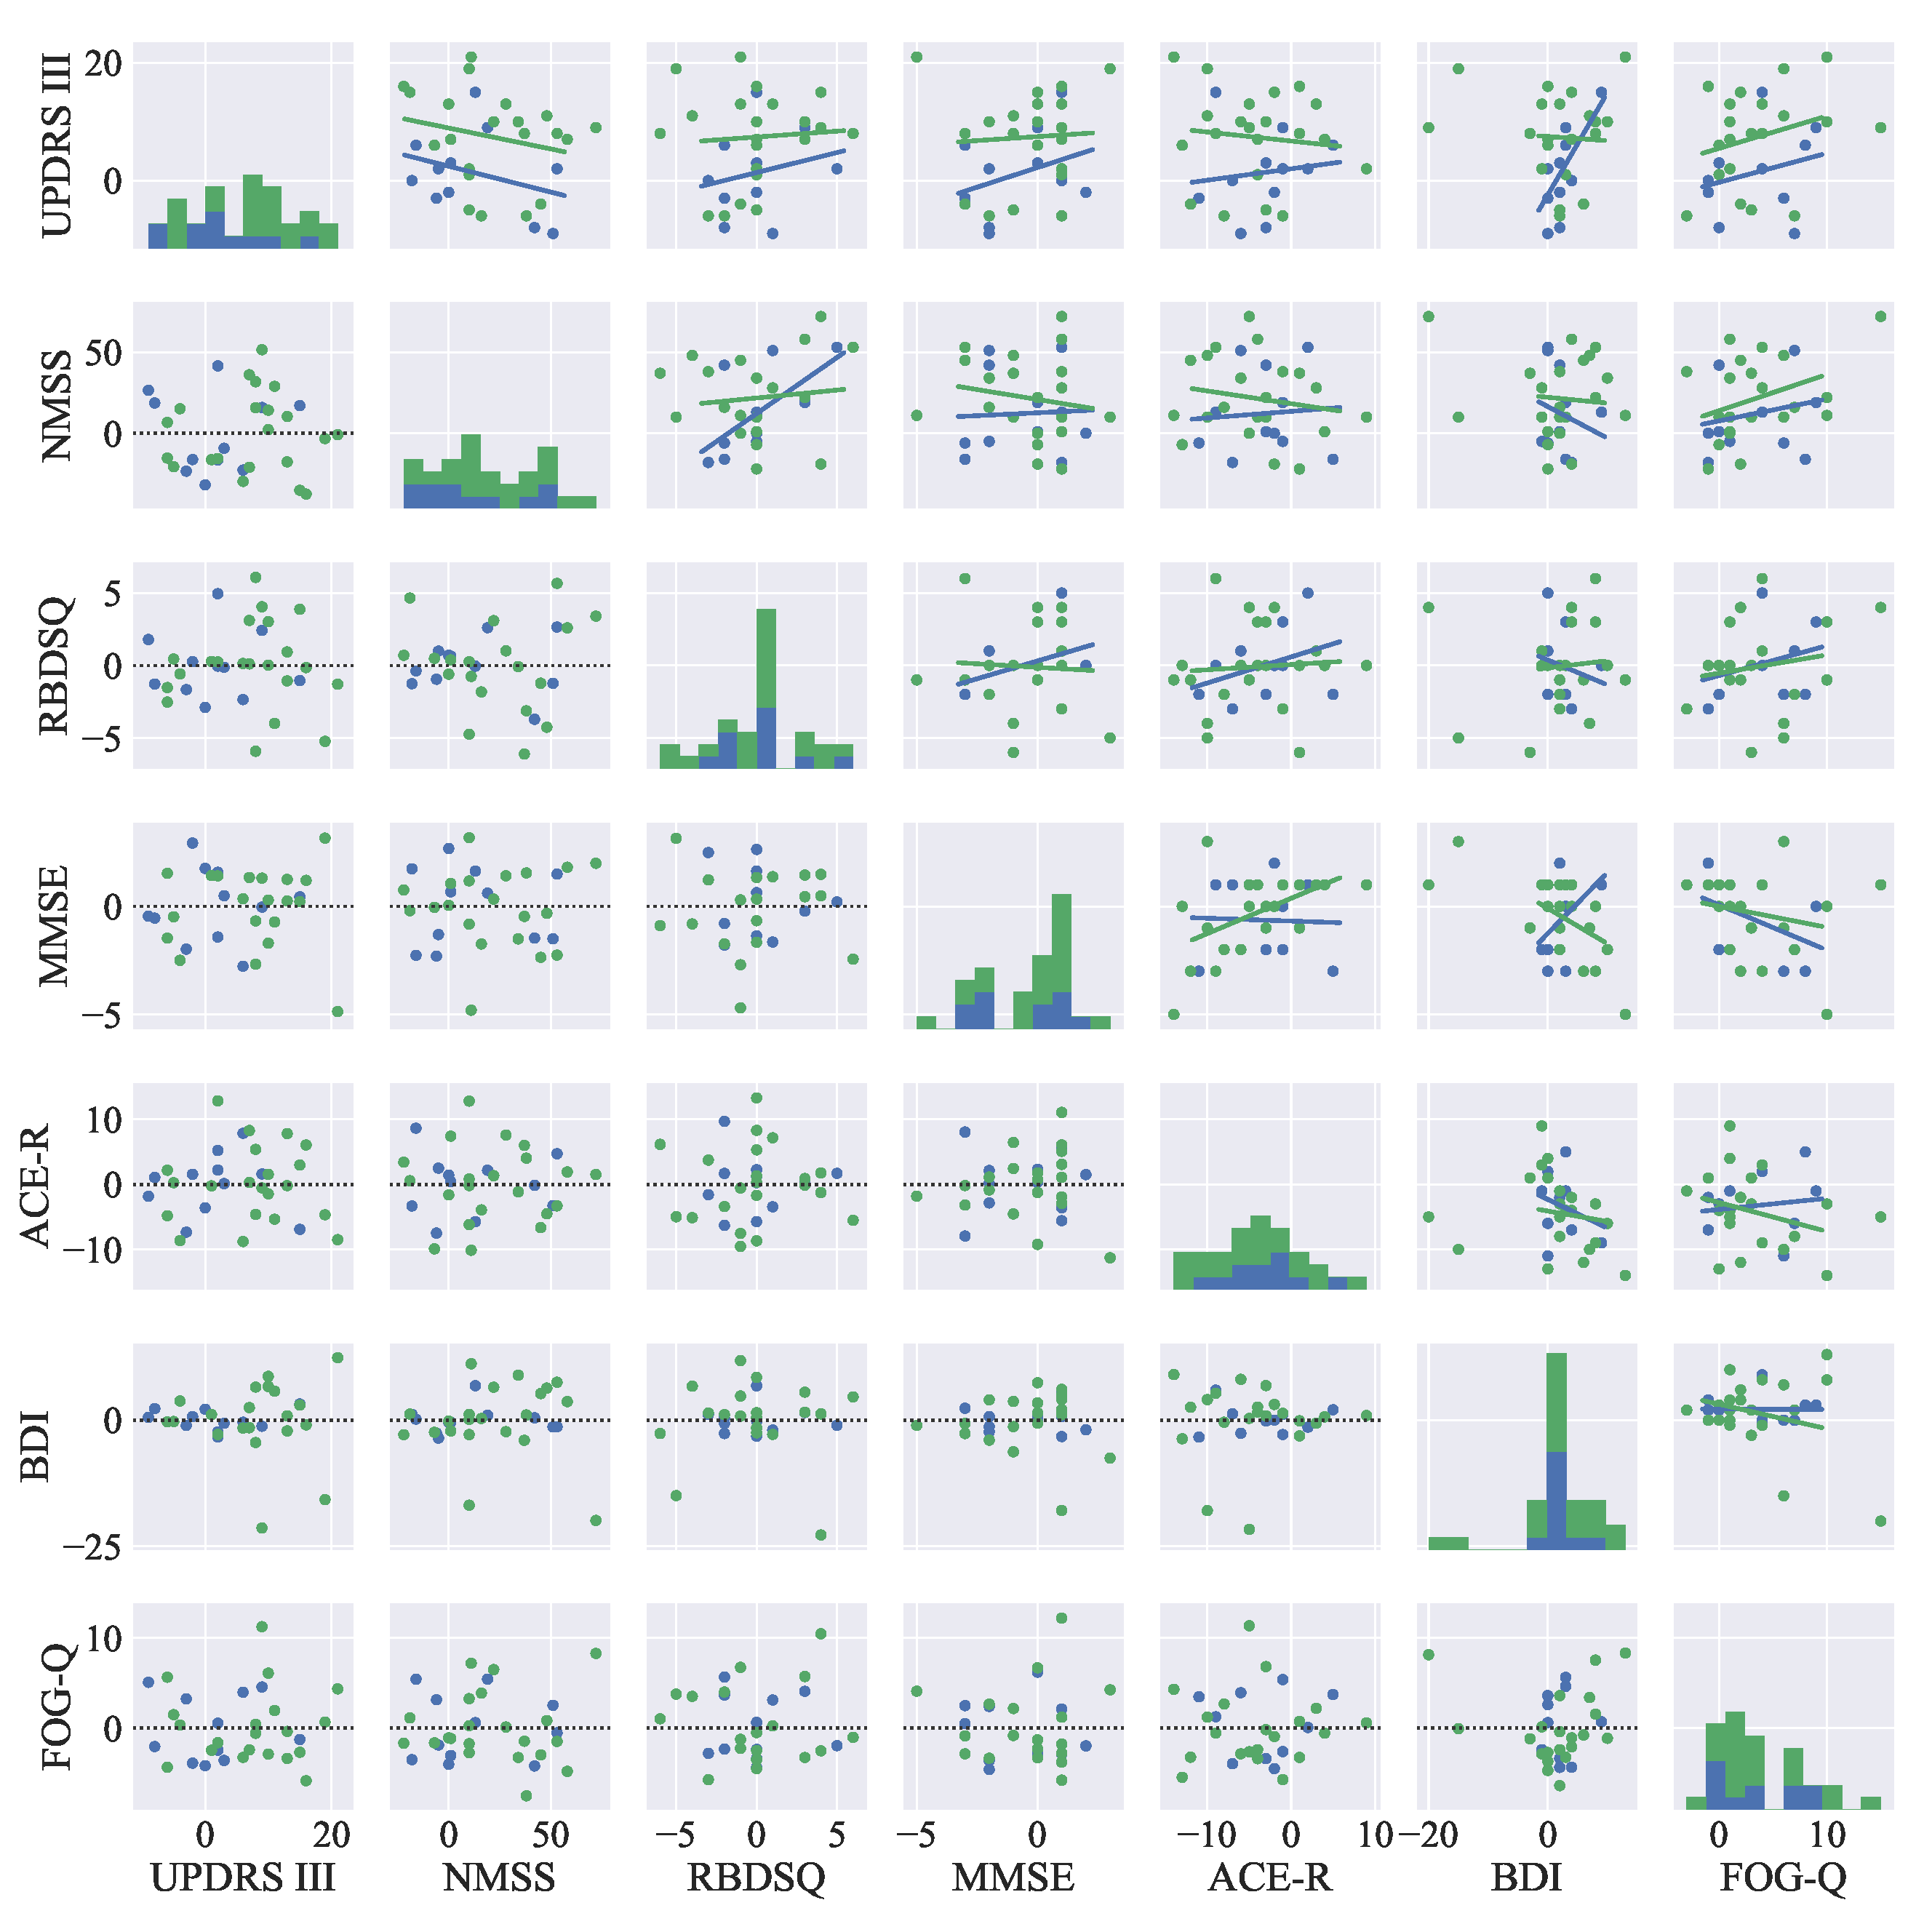
\includegraphics[width=0.99\textwidth]{pictures/ch6_clinical_statistics.eps}
	\caption[Descriptive statistical graphs of clinical data for PD patients.]{Descriptive statistical graphs of clinical characteristics of PD patients participated in this study (data for the $\delta$ session ($\mbox{session 2} - \mbox{session 1}$) only): on the main diagonal, histograms are visualized. Next, the upper triangular part of the graph-grid shows scatter plots with the fitted lines of the linear regression models. And finally, the lower triangular part of the graph-grid is used to display residuals for the models shown in the the upper grid. Colour notation: blue colour represents female speakers, and green colour represents male speakers. For the description of the rating scales, see Table~\ref{tab:ch6_clinical_data}}
	\label{fig:ch6_clinical_statistics}
\end{figure}

\newpage
With respect to the assessment of gait freezing, every patient was examined by a~trained movement disorders specialist who rated the gait-related difficulties according to a~specialized six-item Likert-scale ($5$-point scale where a~score of $0$ indicates absence of the symptom, while a~score of $4$~indicates the most severe stage; therefore the total score ranges from $0$--$24$): Freezing of gait questionnaire~\cite{Giladi2000}. Full template can be seen in Appendix~\ref{tab:FOGQ_template}. The scale can be theoretically divided into two parts: 1st part (question\,$1$--question\,$2$) assesses walking and gait-related difficulties affecting patient's daily activities and independence; 2nd part (question\,$3$--question\,$6$) assesses gait freezing specifically. There is also a~total score (T) computed as a~sum of the two sub-scores ($\mbox{T}_1$ for Q1--Q2, and $\mbox{T}_2$ for Q3--Q6) summarizing the two parts ($\mbox{T} = \mbox{T}_1 + \mbox{T}_2$, where $\mbox{T}_1 = \mbox{Q1} + \mbox{Q2}$, and $\mbox{T}_2 = \mbox{Q3} + \mbox{Q4} + \mbox{Q5} + \mbox{Q6}$). This study was focused on gait freezing exclusively, therefore only the second part of the questionnaire and its total score are considered.

Furthermore, to provide more insight into the evolution of gait-related deficits (specifically Q6--Q6 score and the total score (sum of Q1--Q6)) between the two examinations (session $1$, and session $2$), box plots are presented as well. These graphs can be seen in Figure~\ref{fig:ch6_boxplots}. For the purpose of this visualization, all samples from both sessions were used (as opposed to the descriptive statistical graphs shown in Figure~\ref{fig:ch6_clinical_statistics} in which only a~subset of speakers with no missing data was selected). The reason behind this is to show a~distribution of the data based on as much observations as possible to better approximate the reality.

\begin{figure}[htb!]
	\centering
	\scriptsize
	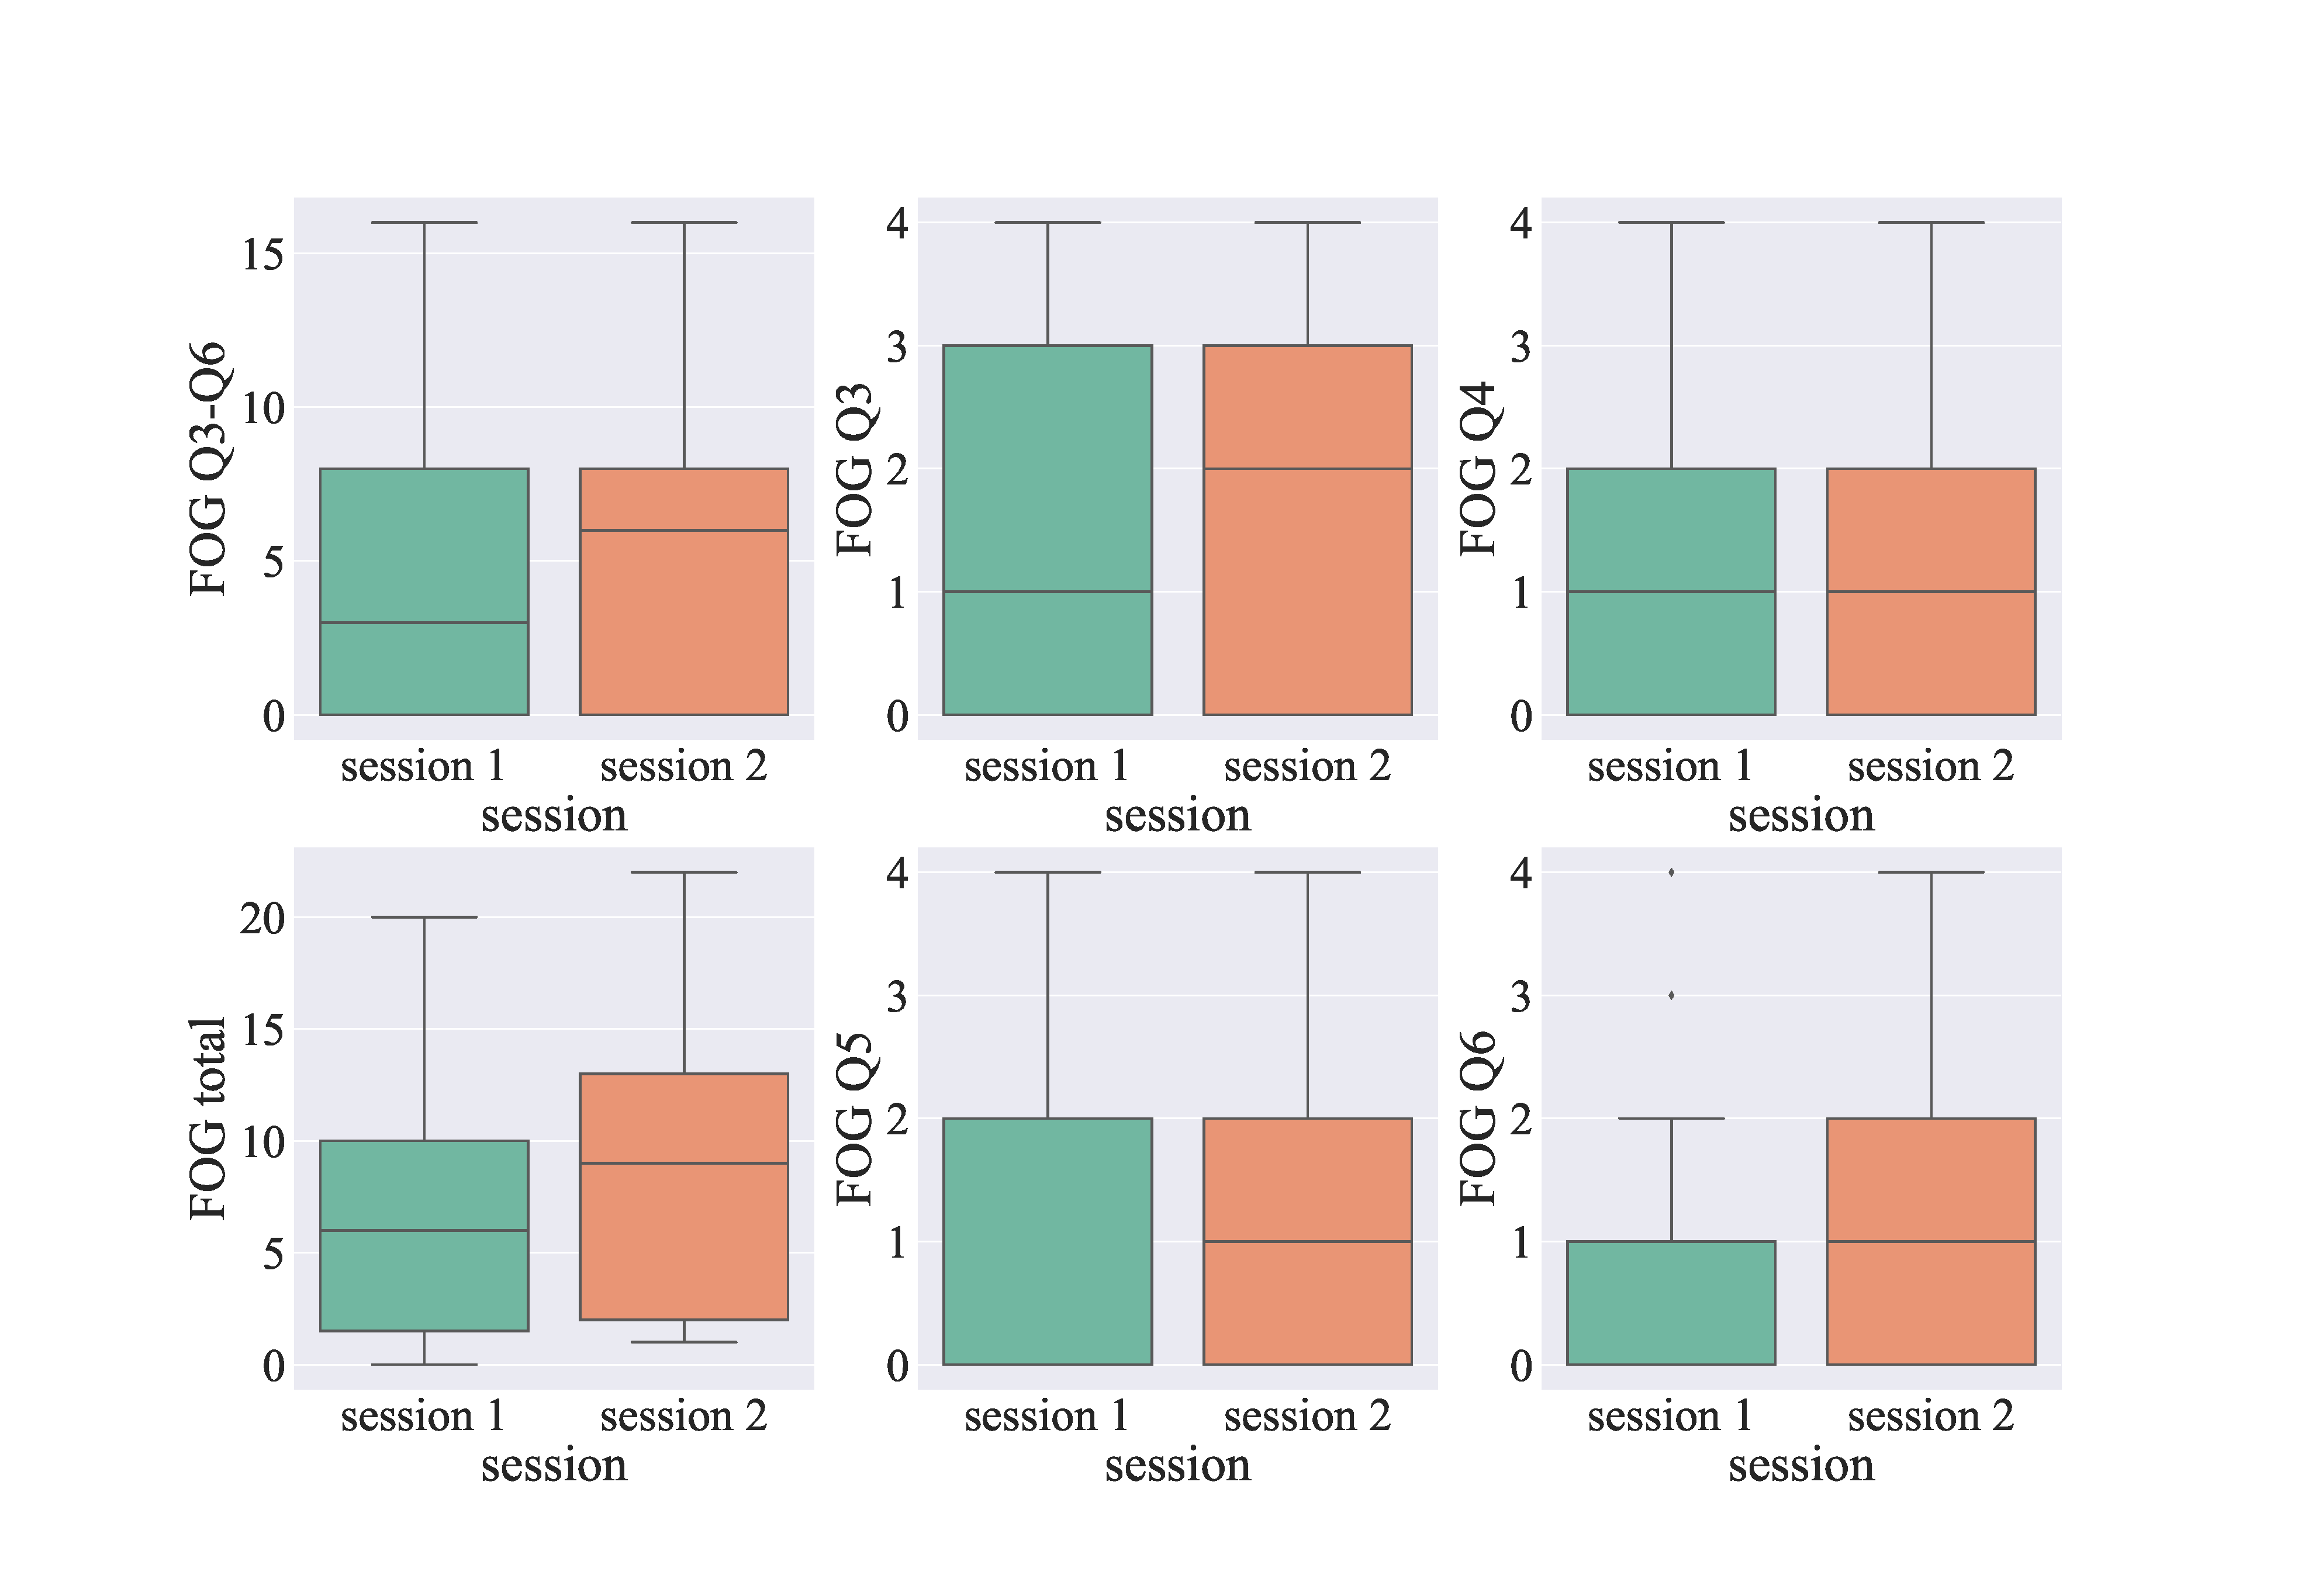
\includegraphics[width=0.99\textwidth]{pictures/ch6_box_plots_clin_fog.eps}
	\caption[Box plots for clinical data (gait assessment).]{Box plots visualizing the evolution of gait-specific deficits assessed by FOG-Q, specifically Q3--Q6 score and the total score (sum of Q1--Q6). Colour notation: green colour represents data for session $1$ (baseline examination), and blue colour represents data for session $2$ (follow-up examination).}
	\label{fig:ch6_boxplots}
\end{figure}

Regarding the speech task used to quantify HD, a~complex set of tasks was used to robustly quantify voice/speech disorders occurring with this disease. The speech acquisition protocol was actually derived from the standardized 3F Dysarthria Profile~\cite{Kostalova2013} and included fourteen speech tasks, specifically: monologue, expiration with closed/open lips, sustained phonation (/a/, /i/), diadochokinesis, rhythmical units, basic intonation/stress templates, and reading with different/no emotions. More complete description of these speech tasks can be seen in Table~\ref{tab:ch6_speech_tasks}. And finally, the actual acquisition of the acoustic signals was performed exactly in the same way as in the other studies summarized in this thesis. For more information, see chapter~\ref{ch4}.

\begin{table*}[htb!]
	\centering
	\begin{threeparttable}
		\caption{List of the examination speech tasks.}
		\label{tab:ch6_speech_tasks}
		\footnotesize
		\centering
		\begin{tabularx}{1.00\textwidth}{l l X}

			\hline\hline\noalign{\smallskip}
			\rowcolor{gray_table}
			label & vocal task & description \\
			\noalign{\smallskip}\hline\noalign{\smallskip}

			T1 & 
			Monologue & 
			Free speech without the interruption of a~clinician. The participants were instructed to speak about their daily living, hobbies, family, an so on. \\
			
			T2 & 
			Expiration with closed lips & 
			Sustained phonation of the consonant /m/ with closed lips as constantly and for as long as possible. It should be performed in one breath if possible. \\
			
			T3 & 
			Expiration with open lips & 
			Sustained phonation of the vowel /i/ with open lips as constantly and for as long as possible. It should be performed in one breath if possible. \\
			
			T4 & 
			Sustained phonation & 
			Sustained phonation of the vowel /a/ at a~comfortable pitch and loudness. Performed in one breath and without any limitations in length. \\
			
			T5 & 
			Diadochokinetic task & 
			Rapid and steady /pa/-/ta/-/ka/ syllable repetition as constantly and for as long as possible. It should be performed in one breath if possible. \\
			
			T6 & 
			Rhythmical units & 
			Reading a~text containing 4 rhymes of 16 words rhythmically (i.\,e. poem recitation, for more information about the task, see description in Chapter~\ref{ch4}). \\
			
			T7 & 
			Basic intonation template & 
			Short sentence reading containing 3 words. The sentence should be pronounced interrogatively (i.\,e. stress-modified reading, similar to Chapter~\ref{ch4}). \\
			
			T8 & 
			Basic intonation template & 
			Short sentence reading containing 3 words. The sentence should be pronounced imperatively (i.\,e. stress-modified reading, similar to Chapter~\ref{ch4}). \\
			
			T9 & 
			Basic intonation template & 
			Short sentence reading containing 3 words. The sentence should be pronounced declaratively (i.\,e. stress-modified reading, similar to Chapter~\ref{ch4}). \\
			
			T10 & 
			Reading paragraph & 
			Reading phonetically unbalanced text of 135 words. \\
			
			T11 & 
			Reading with different emotions & 
			Reading a~sentence of 8 words neutrally. \\
			
			T12 & 
			Reading with different emotions & 
			Reading a~sentence of 6 words angrily. \\
			
			T13 & 
			Reading with different emotions & 
			Reading a~sentence of 9 words in a~bored manner. \\
			
			T14 & 
			Reading with different emotions & 
			Reading a~sentence of 5 words excitedly. \\

			\noalign{\smallskip}\hline\hline
		\end{tabularx}
	\end{threeparttable}
\end{table*}

\subsection{Feature extraction}
\label{ch6_3_2}

To quantify voice/speech disorders in the PD patients, a~set of acoustic features based on a~recommendation given in recent review on acoustic analysis of voice/speech signals in patients suffering from HD~\cite{Brabenec2017} was computed. It specifically covers the area of phonation (Appendix~\ref{tab:phonatory_features}), articulation (Appendix~\ref{tab:articulation_features}), and prosody (Appendix~\ref{tab:prosodic_features}). To provide better insight into ability of these features to describe HD, a~short description per HD area is presented.

In terms of phonation, the acoustic features describing airflow insufficiency (MPT) during expiration with closed (T2) or opened (T3) lips, irregular pitch fluctuations (relF0SD) during phonation of the vowel /a/ (T4), microperturbations in frequency (jitter) and amplitude (shimmer) during phonation of the vowel /a/ (T4), tremor of jaw (F1SD, F2SD) during phonation of the vowel /a/ (T4), increased acoustic noise (mean HNR) during phonation of the vowel /a/ (T4), and aperiodicity of voice (DUV) during phonation of the vowel /a/ (T4) were computed.

With respect to articulation, the acoustic features describing rigidity of tongue and jaw (F1IR, F2IR, F1SD, F2SD) during monologue (T1), rhythmical reading (T6), basic intonation templates (T7--9), paragraph reading (T10), and reading with different emotions (T11--14), slow alternating motion rate (DDK rate) during diadochokinetic task (T5), and irregular alternating motion rate (DDK reg) during diadochokinetic task (T5) were computed.

Finally, regarding the acoustic features describing monopitch (relF0SD) and monoloudness (relSEOSD) during monologue (T1), rhythmical reading (T6), basic intonation templates (T7--9), paragraph reading (T10), and reading with different emotions (T11--14), inappropriate silences (SPIR) during paragraph reading (T10), unnatural speech rate (TSR, NSR) during basic intonation templates (T7--9), paragraph reading (T10), and reading with different emotions (T11--14) were computed.

\subsection{Analytical setup}
\label{ch6_3_3}

To assess the strength of a~relationship between the patients' clinical data and the selected items of FOG-Q in both sessions (session $1$, session $2$), Pearson's correlation with the significance level $0.05$ was used. With this approach, it was possible to identify those clinical measures (PD duration, UPDRS~III, LED (mg/day), NMSS, RBDSQ, MMSE, ACE-R, BDI) that are significantly correlated with the specific symptoms of gait freezing in PD, which is a~very valuable information because it shows which clinical aspects of PD tend to be associated with FOG in the baseline and in the follow-up (after $2$ years). Using the $\delta$ session ($\mbox{session 2} - \mbox{session 1}$), it is even possible to see if the evolution of other clinical aspects of PD is related with the evolution of the associated gait problems.

Next, to assess the strength of a~relationship between voice/speech disorders in HD and freezing of gait in patients with PD, Pearson's (linear relationship) and Spearman's (monotonic relationship) partial correlation coefficients\footnote{Partial correlation measures the unbiased degree of association between two variables while controlling for the effect of other confounding factors (variables).} between the acoustic features and the values of FOG-Q were computed. The significance level of correlation in this case was set to $0.05$ as well. During the computation of partial correlations, the factors such as patients' age and gender \cite{Skodda2011d, Vergara2017}, dopaminergic medication~\cite{Lee2010} and a~variety of associated motor and non-motor symptoms assessed by UPDRS~III~\cite{Fahn1987}, BDI \cite{Beck2000, Beck1961}, and ACE-R~\cite{Larner2007} were controlled for. As in the previous case, the aim was to identify those acoustic features that are significantly correlated with the specific symptoms of gait freezing in PD.

Finally, to evaluate the power of the acoustic features (in session $1$; baseline) in predicting the change of the severity of gait freezing in PD ($\Delta\,\mbox{FOG-Q}$), multivariate regression analysis was performed. For this purpose, we employed classification and regression trees (CART) in the supervised machine learning setup using stratified $10$-fold cross-validation with $100$ repetitions)~\cite{Breiman1984}. As previously, see Chapter~\ref{ch4} and Chapter~\ref{ch5}, feature selection process was applied to obtain the feature sets with the maximum clinical interpretability and also the power to predict FOG-related deficits in patients with PD. For this purpose, a~modified version of sequential floating forward selection~\cite{Pohjalainen2014} algorithm was used. To evaluate the prediction performance of the trained models, mean absolute error (MAE), root mean squared error (RMSE), and estimation error rate (EER) were computed. For more information about these metrics, see Chapter~\ref{ch5}.

\section{Results}
\label{ch6_4}

Regarding the classical correlation analysis, the values of Pearson's correlation coefficients computed between clinical data (e.\,g. scores of the clinical rating scales assessing motor and non-motor symptoms of PD) and selected items of FOG-Q (i.\,e. Q3--Q6, and the total score) can be found in Table~\ref{tab:ch6_classical_correlations}. This type of correlation was computed for all three sessions: session $1$ (baseline examination), session $2$ (follow-up examination), and $\delta$ session (description of the change in the particular item of the rating scale) The results are discussed bellow.

\begin{table*}[htb!]
	\centering
	\begin{threeparttable}
		\caption{Correlations among patients' FOG-Q items and clinical description.}
		\label{tab:ch6_classical_correlations}
		\footnotesize
		\centering
		\begin{tabular}{l r c r c r c r c r c}

			\hline\hline\noalign{\smallskip}
			\rowcolor{gray_table}
			FOG-Q & $\rho$\,(Q3) & $p$ & $\rho$\,(Q4) & $p$ & $\rho$\,(Q5) & $p$ & $\rho$\,(Q6) & $p$ & $\rho$\,(total) & $p$ \\
			\noalign{\smallskip}
			\multicolumn{11}{c}{Session 1} \\
			\noalign{\smallskip}\hline\noalign{\smallskip}

			PD dur. (years)  &  0.47 & ** &  0.35 & ** &  0.35 & ** &  0.39 & ** &  0.44 & ** \\
			UPDRS III        &  0.24 & *  &  0.24 & *  &  0.24 &    &  0.23 & *  &  0.25 & *  \\
			LED (mg/day)     &  0.36 & ** &  0.33 & ** &  0.37 & ** &  0.24 & *  &  0.37 & ** \\
			NMSS             &  0.45 & ** &  0.43 & ** &  0.39 & ** &  0.52 & ** &  0.49 & ** \\
			RBDSQ            &  0.25 & *  &  0.28 & *  &  0.14 &    &  0.28 & *  &  0.27 & *  \\
			MMSE             & -0.01 &    & -0.07 &    &  0.06 &    & -0.06 &    & -0.02 &    \\
			ACE-R            & -0.06 &    & -0.15 &    &  0.04 &    & -0.13 &    & -0.08 &    \\
			BDI              &  0.05 &    &  0.06 &    &  0.09 &    &  0.13 &    &  0.09 &    \\

			\noalign{\smallskip}\hline\noalign{\smallskip}
			\multicolumn{11}{c}{Session 2} \\
			\noalign{\smallskip}\hline\noalign{\smallskip}

			PD dur. (years)  &  0.41 & ** &  0.41 & ** &  0.38 & ** &  0.42 & ** &  0.44 & ** \\
			UPDRS III        &  0.36 & *  &  0.45 & ** &  0.35 & *  &  0.39 & *  &  0.42 & ** \\
			LED (mg/day)     &  0.28 &    &  0.03 &    &  0.17 &    &  0.15 &    &  0.18 &    \\
			NMSS             &  0.39 & *  &  0.30 &    &  0.26 &    &  0.36 & *  &  0.36 & *  \\
			RBDSQ            &  0.34 & *  &  0.28 &    &  0.38 & *  &  0.41 & ** &  0.38 & *  \\
			MMSE             & -0.26 &    & -0.14 &    & -0.14 &    & -0.07 &    & -0.17 &    \\
			ACE-R            & -0.25 &    & -0.18 &    & -0.18 &    & -0.13 &    & -0.20 &    \\
			BDI              &  0.36 & *  &  0.36 & *  &  0.38 & *  &  0.38 & *  &  0.40 & ** \\

			\noalign{\smallskip}\hline\noalign{\smallskip}
			\multicolumn{11}{c}{$\Delta$ (Session 2 $-$ Session 1)} \\
			\noalign{\smallskip}\hline\noalign{\smallskip}

			PD dur. (years)  & -0.22 &    &  0.06 &    &  0.18 &    &  0.25 &    &  0.04 &    \\
			UPDRS III        &  0.03 &    &  0.17 &    &  0.17 &    &  0.10 &    &  0.16 &    \\
			LED (mg/day)     & -0.28 &    & -0.33 &    & -0.35 &    & -0.18 &    & -0.40 & *  \\
			NMSS             &  0.20 &    &  0.04 &    &  0.20 &    &  0.42 & *  &  0.28 &    \\
			RBDSQ            &  0.09 &    &  0.24 &    &  0.06 &    &  0.24 &    &  0.21 &    \\
			MMSE             & -0.35 & *  & -0.26 &    & -0.29 &    & -0.12 &    & -0.36 & *  \\
			ACE-R            & -0.17 &    & -0.25 &    & -0.24 &    & -0.06 &    & -0.25 &    \\
			BDI              & -0.26 &    & -0.10 &    & -0.06 &    &  0.02 &    & -0.16 &    \\

			\noalign{\smallskip}\hline\hline
		\end{tabular}

		\begin{tablenotes}
			\scriptsize
			\item[1] Table notation: $\rho$\,--\,Spearman's correlation coefficient; $p$\,--\,significance level of correlation (* means $p<0.05$; ** means $p<0.01$); UPDRS~III\,--\,Unified Parkinson's disease rating scale, part~III: evaluation of motor function~\cite{Fahn1987}; LED\,--\,L-dopa equivalent daily dose~\cite{Lee2010}; NMSS\,--\,Non-motor symptoms scale~\cite{Chaudhuri2007}; RBDSQ\,--\,The REM sleep behavior disorder screening questionnaire~\cite{Stiasny2007}; MMSE\,--\,Mini-mental state examination~\cite{Folstein1975}; ACE-R\,--\,Addenbrooke's cognitive examination-revised~\cite{Larner2007}; BDI\,--\,Beck depression inventory \cite{Beck2000, Beck1961}; FOG-Q\,--\,Freezing of gait questionnaire~\cite{Giladi2000} (Q1--Q6, and T\,--\,total score), for more details, see Section~\ref{tab:ch6_clinical_data}.
		\end{tablenotes}
	\end{threeparttable}
\end{table*}

In both sessions, significant correlations of all FOG-Q items with duration of PD and UPDRS~III (except Q5 in session $1$) were identified. Next, LED was found significantly correlated with all FOG-Q items in session $1$, but not in the session $2$. Next, NMSS and all items of FOG-Q were found significantly correlated in session $1$, however in the session $2$ only few significant correlations were found. Regarding RBDSQ, no specific pattern can be observed. FOG-Q items correlated variably with RBDSQ, however, significant correlation for FOG-Q (total score) was found in both sessions. The scales assessing cognitive functions (MMSE, ACE-R) were not find significantly correlated with the items of FOG-Q. And finally, BDI score was not found significantly correlated with FOG-Q in session $1$. Nevertheless, significant correlations can be observed in session $2$. Regarding the correlations between $\Delta\,(\mbox{Q3--6, total score})$ and $\Delta$ of the clinical scores, significant correlations between the changes in FOG-Q items and changes in LED, NMSS and MMSE were identified. Next, the results for partial correlation analysis are summarized in Table~\ref{tab:ch6_partial_correlations}. The associated regression plots can be seen in Figure~\ref{fig:ch6_correlation_plots}.

\begin{table*}[htb!]
\centering
	\begin{threeparttable}
		\caption{Partial correlations among features and FOG-Q (session 1) items.}
		\label{tab:ch6_partial_correlations}
		\footnotesize
		\centering
		\begin{tabular}{l l l r c r c}
			
			\hline\hline\noalign{\smallskip}
			\rowcolor{gray_table}
			HD area & specific disorder & features & $\rho$\,(P) & $p$\,(P) & $\rho$\,(S) & $p$\,(S) \\
			\noalign{\smallskip}
			\multicolumn{7}{c}{FOG\,(Q3)} \\
			\noalign{\smallskip}\hline\noalign{\smallskip}

			prosody      & unnatural speech rate      & NSR\,(T8)   &  0.41 & ** &  0.34 & *  \\
			articulation & rigidity of tongue and jaw & F1IR\,(T10) & -0.40 & ** & -0.44 & ** \\
			articulation & rigidity of tongue and jaw & F1IR\,(T9)  & -0.34 & *  & -0.38 & ** \\
			articulation & rigidity of tongue and jaw & F1IR\,(T13) & -0.32 & *  & -0.39 & ** \\
			articulation & rigidity of tongue and jaw & F1IR\,(T14) & -0.30 & *  & -0.30 & *  \\
			articulation & rigidity of tongue and jaw & F1IR\,(T7)  & -0.30 & *  & -0.35 & *  \\
			
			\noalign{\smallskip}\hline\noalign{\smallskip}
			\multicolumn{7}{c}{FOG\,(Q4)} \\
			\noalign{\smallskip}\hline\noalign{\smallskip}

			articulation & rigidity of tongue and jaw & F1IR\,(T10) & -0.40 & ** & -0.43 & ** \\
			articulation & rigidity of tongue and jaw & F1IR\,(T9)  & -0.35 & *  & -0.40 & ** \\
			
			\noalign{\smallskip}\hline\noalign{\smallskip}
			\multicolumn{7}{c}{FOG\,(Q5)} \\
			\noalign{\smallskip}\hline\noalign{\smallskip}

			articulation & rigidity of tongue and jaw & F1IR\,(T14) & -0.47 & ** & -0.49 & ** \\
			prosody      & unnatural speech rate      & NSR\,(T8)   &  0.36 & *  &  0.42 & ** \\
			articulation & rigidity of tongue and jaw & F1IR\,(T10) & -0.36 & *  & -0.40 & ** \\
			articulation & rigidity of tongue and jaw & F1IR\,(T13) & -0.29 & *  & -0.36 & *  \\
			
			\noalign{\smallskip}\hline\noalign{\smallskip}
			\multicolumn{7}{c}{FOG\,(Q6)} \\
			\noalign{\smallskip}\hline\noalign{\smallskip}

			prosody      & unnatural speech rate      & TSR\,(T11)  &  0.33 & *  &  0.33 & *  \\
			prosody      & unnatural speech rate      & NSR\,(T8)   &  0.33 & *  &  0.33 & *  \\
			prosody      & unnatural speech rate      & NSR\,(T11)  &  0.32 & *  &  0.32 & *  \\

			\noalign{\smallskip}\hline\noalign{\smallskip}
			\multicolumn{7}{c}{FOG\,(total score)} \\
			\noalign{\smallskip}\hline\noalign{\smallskip}

			articulation & rigidity of tongue and jaw & F1IR\,(T10) & -0.40 & ** & -0.45 & ** \\
			articulation & rigidity of tongue and jaw & F1IR\,(T14) & -0.38 & ** & -0.38 & ** \\
			articulation & unnatural speech rate      & NSR\,(T8)   &  0.36 & *  &  0.38 & ** \\
			
			\noalign{\smallskip}\hline\hline
		\end{tabular}
	
		\begin{tablenotes}
			\scriptsize
			\item[1] Table notation: $\rho$\,(P)\,--\,Pearson's correlation coefficient; $p$\,(S)\,--\,significance level of correlation according to $\rho$\,(P); $\rho$\,(S)\,--\,Spearman's correlation coefficient; $p$\,(S)\,--\,significance level of correlation according to $\rho$\,(S) (* means $p<0.05$; ** means $p<0.01$); FOG-Q\,--\,Freezing of gait questionnaire~\cite{Giladi2000}.
		\end{tablenotes}
	\end{threeparttable}
\end{table*}

\begin{figure}[htb!]
	\centering
	\scriptsize
	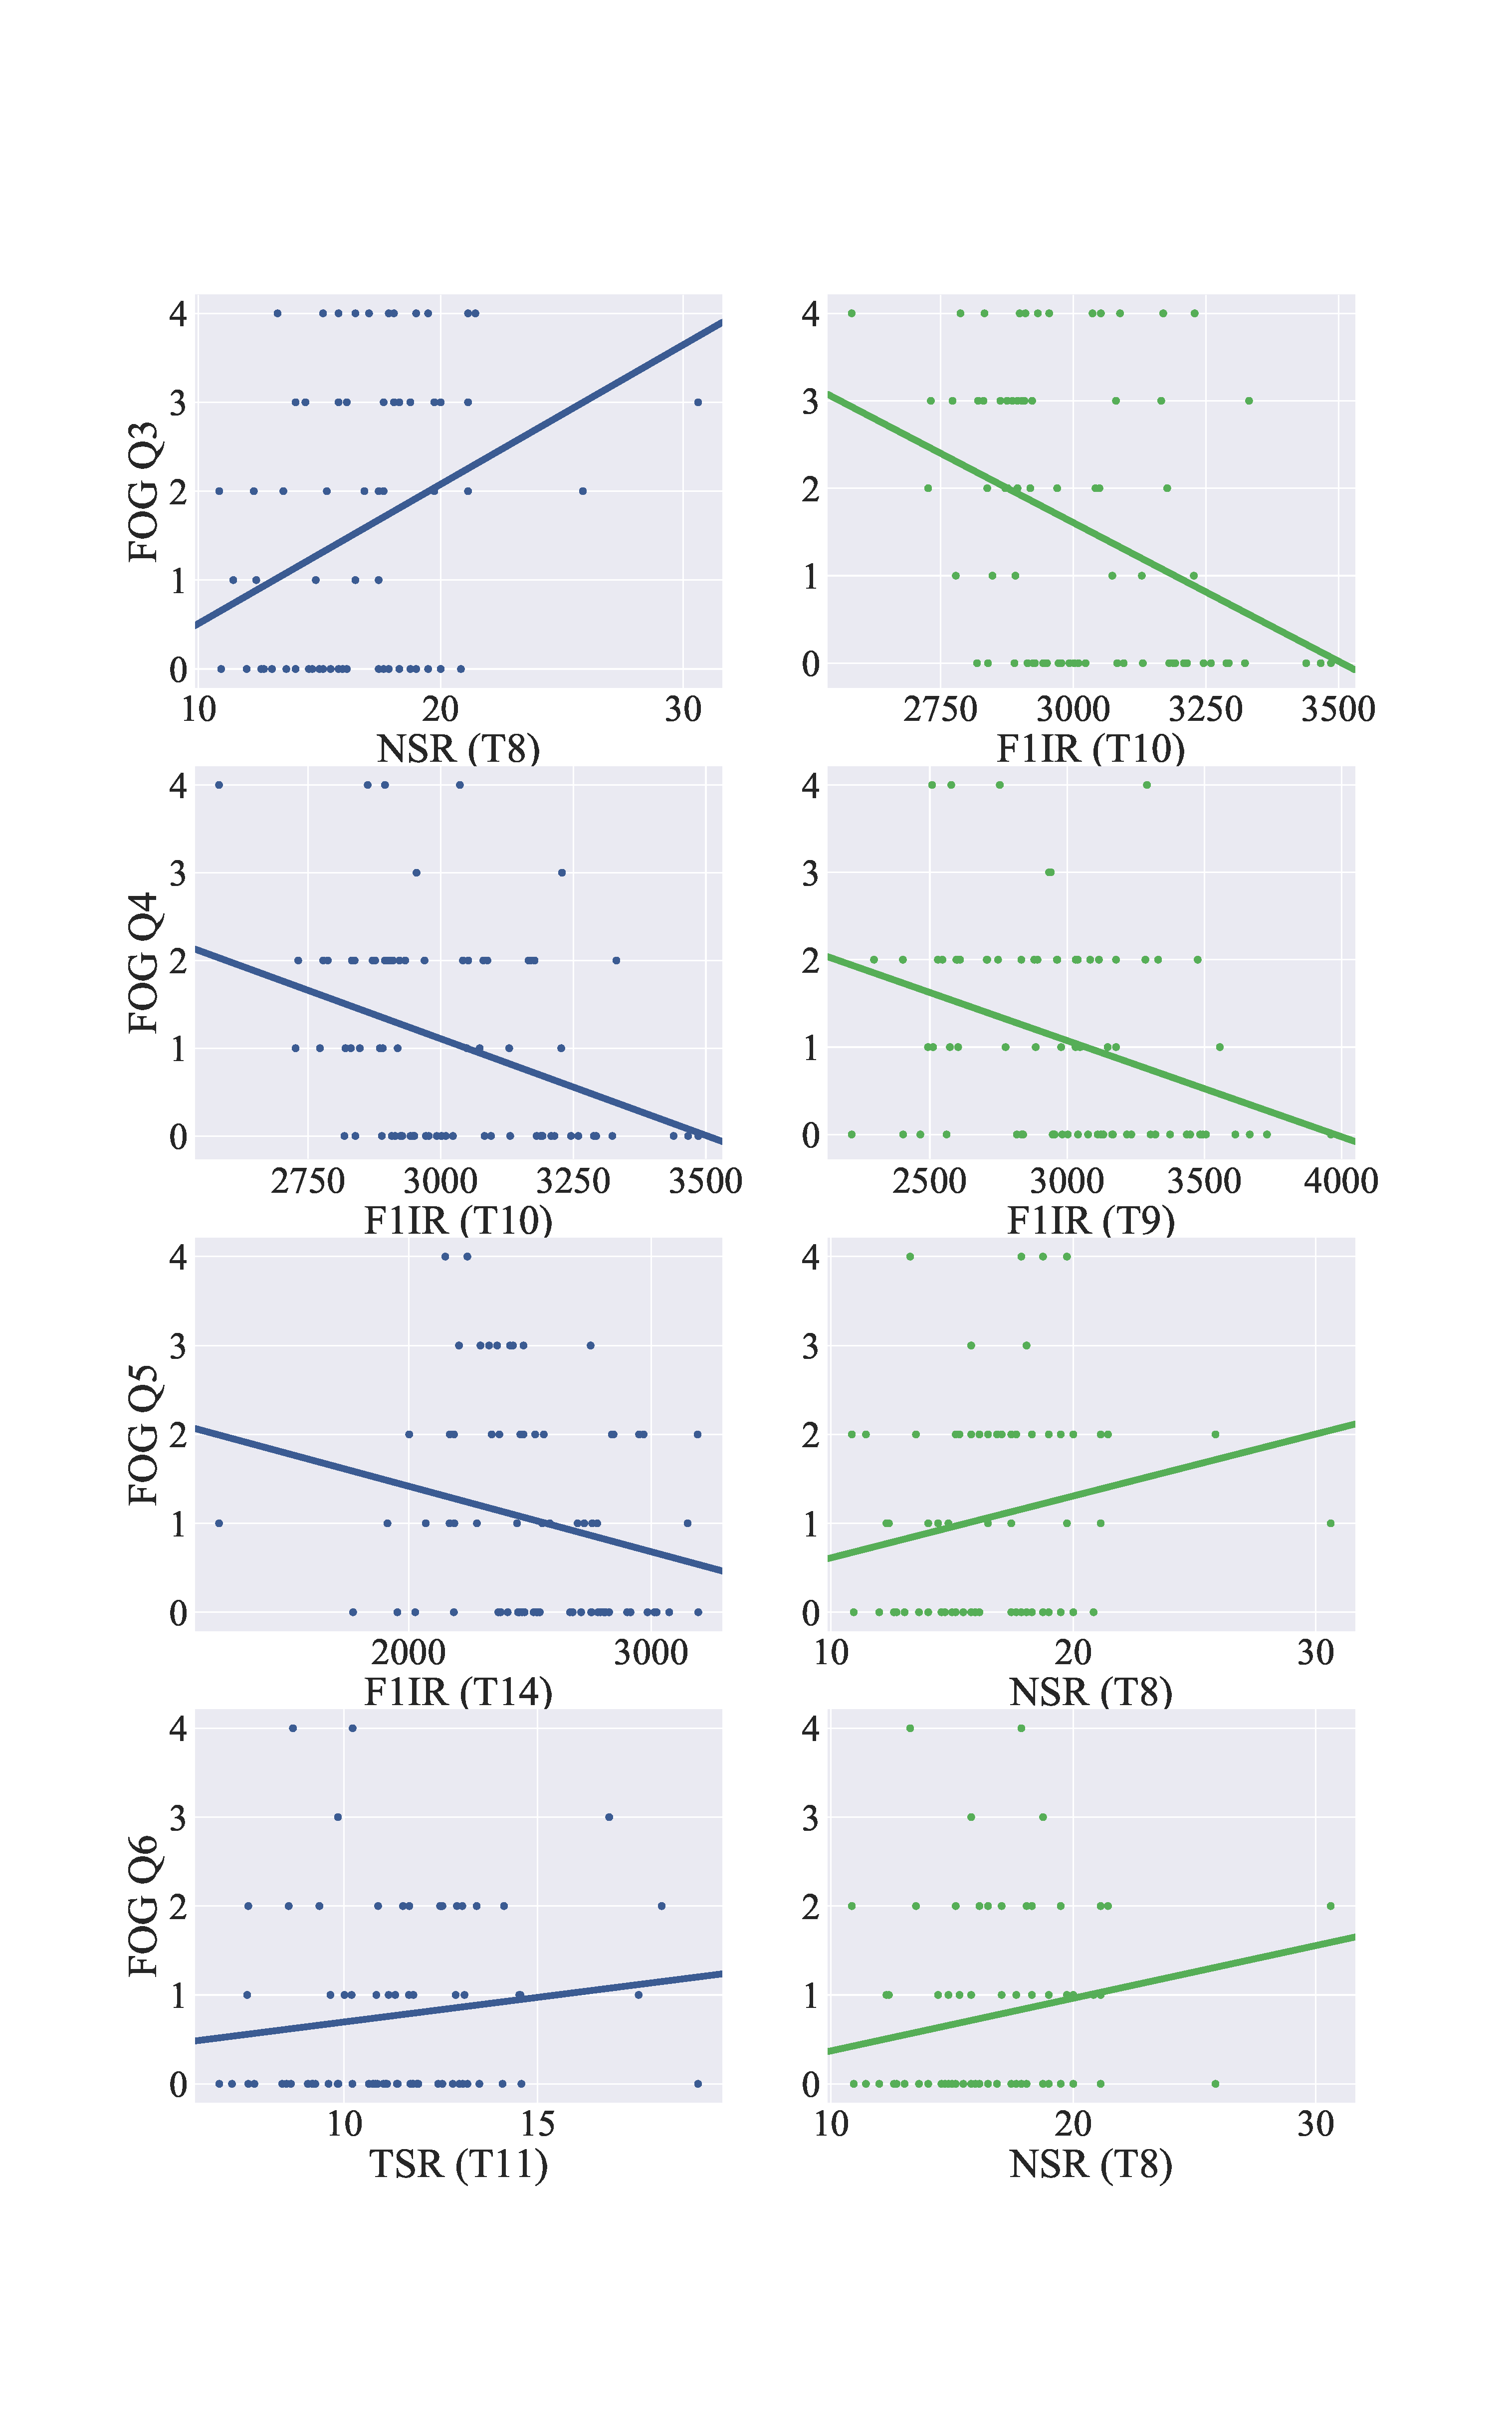
\includegraphics[width=0.80\textwidth]{pictures/ch6_correlation_plots.eps}
	\caption[Regression plots for FOG-Q (Q3--Q6).]{Regression plots (scatter plots with the fitted line of the robust linear regression estimator) of the most correlated acoustic features (partial correlation) for Q3--Q6, see Table~\ref{tab:ch6_partial_correlations}. Colour notation: blue colour represents the most correlated feature; and green colour represents the second most correlated feature. For speech task notation, see Table~\ref{tab:ch6_speech_tasks}.}
	\label{fig:ch6_correlation_plots}
\end{figure}

With respect to the partial correlation analysis, the correlations among acoustic features quantifying impaired phonation, articulation and prosody, and selected items of FOG-Q (Q3--Q6, and the total score) were computed. It is important to point out that the partial correlation analysis was performed for session $1$ only to focus on the investigation of the relationship between FOG and HD in the baseline. For a~better overview, only the acoustic features with significant correlation in both Pearson's, and Spearman's correlations were selected. Regarding Q3 (assessment of occurrence of freezing), this item was found correlated mostly with the interpercentile range of the first formant, and with net speech rate (extracted from reading of a~short sentence). The strongest correlation can be seen in the case of NSR extracted from the short imperative sentence reading ($\rho\,(\mbox{P})=-0.40$, $p<0.01$, and $\rho\,(\mbox{S})=-0.44$, $p<0.01$). In the case of Q4 (assessment of the duration of the longest freezing episode), $2$ significant negative correlations were identified for the interpercentile range of the first formant (extracted from paragraph reading, and short declarative sentence reading). The strongest correlation can be seen in the case of paragraph reading ($\rho\,(\mbox{P})=-0.40$, $p<0.01$, and $\rho\,(\mbox{S})=-0.43$, $p<0.01$). With respect to Q5 (assessment of the duration of the typical start hesitation), the interpercentile range of the first formant (extracted from paragraph reading, reading of $9$ words in a~bored manner, reading of $5$ words excitedly), and with the net speech rate (extracted from short imperative sentence reading) were found significantly correlated with this particular item of the questionnaire. The strongest correlation can be seen in the case of F1IR extracted from the reading of $5$ words in an~excited manner ($\rho\,(\mbox{P})=-0.47$, $p<0.01$, and $\rho\,(\mbox{S})=-0.49$, $p<0.01$). In the case of Q6 (assessment of the duration of the typical turning hesitation), significant correlations were found for total speech rate (extracted from reading of a~sentence of $8$ words in a~neutral manner) and net speech rate (extracted from short imperative sentence reading and reading of a~sentence of $8$ words in a~neutral manner). The strongest correlation can be seen in the case of TSR extracted from the reading of a~sentence of $8$ words in a~neutral manner ($\rho\,(\mbox{P})=0.33$, $p<0.05$, and $\rho\,(\mbox{S})=0.33$, $p<0.05$). And finally, with respect to the total score (Q3--Q6), interpercentile range of the first formant (extracted from paragraph reading and reading of $5$ words excitedly), and net speech rate (extracted from short imperative sentence reading) were found significantly correlated with this item. The strongest correlation can be seen in the case of F1IR extracted from the paragraph reading ($\rho\,(\mbox{P})=-0.40$, $p<0.05$, and $\rho\,(\mbox{S})=-0.45$, $p<0.05$). Next, the results of the multivariate regression analysis can be seen in Table~\ref{tab:ch6_regression_analysis}. Moreover, the models for FOG-G (Q5), and FOG (Q6) are visualized (visualization of the approximation of decision making performed by the regression tree) using the three graphs, see Figure~\ref{fig:ch6_regression_tree_fogq5}, and Figure~\ref{fig:ch6_regression_tree_fogq6}, respectively.

\begin{table*}[htb!]
\centering
	\begin{threeparttable}
		\caption{FOG deficits prediction using classification and regression trees.}
		\label{tab:ch6_regression_analysis}
		\footnotesize
		\centering
		\begin{tabular}{l r r r c l}
			
			\hline\hline\noalign{\smallskip}
			\rowcolor{gray_table}
			FOG-Q & MAE & RMSE & EER & No. & selected features \\
			\noalign{\smallskip}
			\multicolumn{6}{c}{Articulation} \\
			\noalign{\smallskip}\hline\noalign{\smallskip}

			Q3 & 0.86~$\pm$~0.26 & 1.03~$\pm$~0.28 & 20.96~$\pm$~6.38 & 1 & F1SD$^{11}$ \\
			Q4 & 0.76~$\pm$~0.28 & 0.89~$\pm$~0.31 & 20.78~$\pm$~7.73 & 2 & F1IR$^{6}$,\,F2SD$^{14}$ \\
			Q5 & 0.49~$\pm$~0.22 & 0.64~$\pm$~0.34 & 10.52~$\pm$~4.67 & 4 & F2SD$^{7}$,\,F1IR$^{11}$,\,F1SD$^{12}$,\,DDKr$^{5}$ \\
			Q6 & 0.60~$\pm$~0.28 & 0.77~$\pm$~0.43 & 13.85~$\pm$~6.41 & 1 & F1SD$^{6}$ \\
			T  & 2.15~$\pm$~0.63 & 2.53~$\pm$~0.73 & 21.89~$\pm$~6.44 & 1 & F1SD$^{9}$ \\

			\noalign{\smallskip}\hline\noalign{\smallskip}
			\multicolumn{6}{c}{Phonation} \\
			\noalign{\smallskip}\hline\noalign{\smallskip}

			Q3 & 1.11~$\pm$~0.30 & 1.29~$\pm$~0.33 & 27.11~$\pm$~7.33 & 1 & jitter$^{4}$ \\
			Q4 & 0.94~$\pm$~0.28 & 1.14~$\pm$~0.31 & 25.84~$\pm$~7.57 & 2 & shimmer$^{4}$,\,jitter$^{4}$ \\
			Q5 & 0.62~$\pm$~0.24 & 0.81~$\pm$~0.33 & 13.42~$\pm$~5.18 & 1 & MPT$^{3}$ \\
			Q6 & 0.60~$\pm$~0.24 & 0.79~$\pm$~0.34 & 13.95~$\pm$~5.57 & 1 & MPT$^{2}$ \\
			T  & 2.32~$\pm$~0.75 & 2.91~$\pm$~0.90 & 23.64~$\pm$~7.63 & 1 & relF0SD$^{4}$ \\

			\noalign{\smallskip}\hline\noalign{\smallskip}
			\multicolumn{6}{c}{Prosody} \\
			\noalign{\smallskip}\hline\noalign{\smallskip}

			Q3 & 0.85~$\pm$~0.33 & 1.04~$\pm$~0.39 & 20.90~$\pm$~8.01 & 3 & TSR$^{11}$,\,TSR$^{10}$,\,relF0SD$^{11}$ \\
			Q4 & 0.80~$\pm$~0.24 & 0.96~$\pm$~0.27 & 21.88~$\pm$~6.69 & 1 & TSR$^{7}$ \\
			Q5 & 0.56~$\pm$~0.22 & 0.71~$\pm$~0.31 & 12.09~$\pm$~4.77 & 3 & relSEOSD$^{9}$,\,SPIR$^{10}$,\,relF0SD$^{1}$ \\
			Q6 & 0.55~$\pm$~0.20 & 0.71~$\pm$~0.26 & 12.75~$\pm$~4.54 & 2 & TSR$^{7}$,\,NSR$^{14}$ \\
			T  & 2.07~$\pm$~0.71 & 2.59~$\pm$~0.88 & 21.10~$\pm$~7.20 & 4 & TSR$^{11}$,\,TSR$^{10}$,\,TSR$^{9}$,\,NSR$^{8}$ \\

			\noalign{\smallskip}\hline\noalign{\smallskip}
			\multicolumn{6}{c}{Combination} \\
			\noalign{\smallskip}\hline\noalign{\smallskip}

			Q3 & 0.83~$\pm$~0.27 & 1.01~$\pm$~0.31 & 20.40~$\pm$~6.73 & 3 & F1SD$^{11}$,\,relF0SD$^{6}$,\,F2IR$^{1}$ \\
			Q4 & 0.76~$\pm$~0.28 & 0.89~$\pm$~0.31 & 20.78~$\pm$~7.73 & 2 & F1IR$^{6}$,\,F2SD$^{14}$ \\
			Q5 & 0.51~$\pm$~0.21 & 0.66~$\pm$~0.32 & 11.03~$\pm$~4.59 & 3 & F2SD$^{7}$,\,relF0SD$^{4}$,\,F2SD$^{12}$ \\
			Q6 & 0.50~$\pm$~0.21 & 0.65~$\pm$~0.29 & 11.73~$\pm$~4.93 & 4 & TSR$^{7}$,\,HNRm$^{4}$,\,F2SD$^{7}$,\,TSR$^{11}$ \\
			T  & 2.00~$\pm$~0.69 & 2.48~$\pm$~0.82 & 20.35~$\pm$~7.08 & 3 & F1SD$^{9}$,\,TSR$^{11}$,\,F1IR$^{6}$ \\
	
			\noalign{\smallskip}\hline\hline
		\end{tabular}
	
		\begin{tablenotes}
		\scriptsize
			\item[1] Table notation: MAE\,--\,mean absolute error; RMSE\,--\,root mean squared error; EER\,--\,relative estimation error rate (mean absolute error divided by the range of actual values of clinical rating scale present in the dataset; expressed in $\%$); No.\,--\,number of selected features; feature$^{x}$\,--\,acoustic feature and the label of the speech task ($x$), see Section~\ref{tab:ch6_clinical_data}; FOG-Q\,--\,Freezing of gait questionnaire~\cite{Giladi2000} (Q3--Q6, and T\,--\,total score), for more details, see Section~\ref{tab:ch6_clinical_data} as well.
		\end{tablenotes}
	\end{threeparttable}
\end{table*}

\begin{figure}[htb!]
	\centering
	\scriptsize
	\includegraphics[width=0.99\textwidth]{pictures/ch6_tree_model_fogq5.pdf}
	\caption[Regression tree graph visualization for FOG-Q (Q5)]{Visualization of the regression tree built to estimate FOG-Q (Q5). The tree was trained using a~single run applied on all data (all speech tasks and all acoustic features) in the dataset for the features selected by the feature selection algorithm (hence the decision making of the tree is an approximation of the behavior responsible for the results summarized in Table~\ref{tab:ch6_regression_analysis}). In the case of this tree, three acoustic features are used: F2SD (T7), relF0SD (T4), and F2SD (T12).}
	\label{fig:ch6_regression_tree_fogq5}
\end{figure}

\begin{figure}[htb!]
	\centering
	\scriptsize
	\includegraphics[width=0.60\textwidth]{pictures/ch6_tree_model_fogq6.pdf}
	\caption[Regression tree graph visualization for FOG-Q (Q6)]{Visualization of the regression tree built to estimate FOG-Q (Q6). The tree was trained using a~single run applied on all data (all speech tasks and all acoustic features) in the dataset for the features selected by the feature selection algorithm (hence the decision making of the tree is an approximation of the behavior responsible for the results summarized in Table~\ref{tab:ch6_regression_analysis}). In the case of this tree, three acoustic features are used: TSR (T7), HNRm (T4), F2SD (T7), and TSR (T11).}
	\label{fig:ch6_regression_tree_fogq6}
\end{figure}

\newpage
Regarding the multivariate regression analysis, the results can be seen in Table~\ref{tab:ch6_regression_analysis}. The table contains the results related to the prediction of the change in FOG severity in a~two-year horizon. When considering the three HD dimensions separately, the following results were achieved. The change in Q3 was predicted with the estimation error of $20.96\,\%$ using $3$ prosodic features. Specifically, TSR (reading of a~sentence of $8$ words in a~neutral manner), TSR (paragraph reading), and relF0SD (reading of a~sentence of $8$ words in a~neutral manner). The change in Q4 was predicted with the estimation error of $20.78\,\%$ using $2$ articulatory features. Specifically, F1IR (rhythmical reading), and F2SD (reading of $5$ words in an~excited manner). The change in Q5 was predicted with the estimation error of $10.52\,\%$ using $4$ articulatory features. Specifically, F2SD (short interrogative sentence reading), F1IR (reading of a~sentence of $8$ words in a~neutral manner), F1SD (reading of a~sentence of $6$ words angrily), and DDKr (diadochokinetic task). The change in Q6 was predicted with the estimation error of $12.75\,\%$ using $2$ prosodic features. Specifically, TSR (short interrogative sentence reading), and NSR (reading of $5$ words in an~excited manner). The change in total score (Q3--Q6) was predicted with the estimation error of $21.10\,\%$ using $4$ prosodic features. Specifically, TSR (reading of a~sentence of $8$ words in a~neutral manner), TSR (paragraph reading), TSR (short declarative sentence reading), and NSR (short imperative sentence reading). And finally, when considering a~combination of the features, the prediction was improved in the case of Q3, Q6, and total score (the difference, i.\,e. improvement is shown [in percentage]): Q3 ($0.56$), Q6 ($1.02$), and total score ($0.75$). However, as can be seen, the improvements are not that significant, which shows a~strong relationship between separate HD areas and specific FOG deficits.

\section{Conclusion}
\label{ch6_5}

Regarding the correlation between the individual items of FOG-Q and other clinical signs of PD assessed by the previously mentioned clinical rating scales, the following conclusions can be drawn. The results proposed in this study (in both sessions) confirm the previous findings of Giladi et al.~\cite{Giladi2000} who reported a~significant correlation between UPDRS~III and FOG-Q. Next, a~strong association between duration of PD and severity of FOG, which is also in accordance with the previous findings \cite{Macht2007, Nilsson2009, Shine2013}, was identified. In addition to that, the results suggest that FOG-Q scores are no longer correlated with dopaminergic medication assessed by LED (mg/day) after the two-year follow-up, which is an interesting finding that points out to the fact that as the disease progresses, the FOG episodes loose their responsiveness to levodopa, or the effect of this medication is not as easily predictable anymore. This is in line with the literature that reports the unresponsiveness of FOG to levodopa as being more prevalent in the more advanced stages of PD, which is hypothesized to be a~consequence of higher importance and influence of other neurotransmitters and pathophysiological mechanisms besides those related to dopaminergic deficits \cite{Espay2012, Vercruysse2014, Xiao2017}. Next, FOG-Q items were found significantly correlated with non-motor symptoms of PD assessed by NMSS, which supports the findings of Zhang et al.~\cite{Zhang2016}, who pointed out the presence of the relationship between FOG and cardiovascular domain of the NMSS. With respect to RBDSQ, the total score of FOG-Q was found strongly related to the level of REM sleep behaviour disorder assessed by this particular rating scale. This is in line with the findings of several studies reporting that increased muscle activity during REM sleep is a~comorbid feature of patients with PD who exhibit FOG \cite{Videnovic2013, Walton2015, Zhang2016}. With respect to other non-motor symptoms of PD assessed by MMSE and ACE-R, none of the correlations were found significant. This is in contradiction with the previous studies that did demonstrate the presence of a~relationship between impaired cognitive functions and FOG \cite{Rektorova2016, Yao2017}. And finally, in the case of BDI, the significant correlations were found only in the follow-up session that is suggesting that the presence of more advanced depressive symptoms (although not severe enough to diagnose the major depressive episode) at the follow-up examination is linked with the progression of PD. This is also in accordance of the previous studies that showed depressive symptoms could be pertinent and significant predictors of FOG in PD \cite{Giladi2001b, Shine2013, Walton2015}.

Next, in the case of the partial correlation analysis between the acoustic features quantifying phonation, articulation and prosody in HD and selected items of FOG-Q, the following conclusions can be drawn. At first, it must be pointed out that no corrections for multiple comparisons was applied since after employing any of the most commonly-used methods for significance level adjustment such as Bonferroni correction~\cite{Weisstein2004} or false discovery rate (FDR)~\cite{Storey2011}, none of the correlations appeared to be significant (none of the p-values were bellow the chosen significance level of $0.05$). However, this is tightly linked to the number of cohorts in the dataset (to be discussed later). Therefore, the results of this analysis must be considered as exploratory and pilot in nature. So, with that in mind, it can be seen that most of the FOG-Q items, showed statistically significant correlation with the articulatory features, more specifically with the interpercentile range of first formant. Moreover, in some cases, standard deviation of the first formant was close to the significance level as well. To discuss this observation in more details, formants are resonances of the oro-naso-pharyngeal tract that are changed mainly by a~position of tongue and jaw \cite{Gomez2017, Gomez2017b, Vergara2017}, where the first formant is influenced by a~vertical position of these articulatory organs. Therefore the interpercentile range of the first formant is related to the limit positions of the jaw and tongue in the vertical direction, and the standard deviation of this acoustic feature is related to the jaw and tongue tremor (when quantifying sustained phonation) or the speed of articulatory organ position change (when quantifying running speech). All the partial correlations with the formant-based features are negative in direction, i.\,e. the worse performance in FOG-Q can in theory be linked to the worse articulation. This confirms the previous findings of Ricciardi et al.~\cite{Ricciardi2016}, who used~a simple one-item articulation analysis using the dysarthria profile. In addition to that, speech rate  (quantified either by the total speech rate or by the net speech rate) was also found significantly correlated with FOG. In contrary to the previously published work of Ricciardi et al.~\cite{Ricciardi2016}, in the frame of this thesis, the positive correlations with FOG-Q items were identified. This suggests that patients with more severe FOG exhibited a~higher speech rate. However, the data also shows that with increasing speech rate the articulation was less precise as well, which could mean that more severe FOG is linked to speech rashes and disturbed and/or less intelligible speech. Furthermore, no significant correlation between vocal tremor and FOG can be observed. This is in contradiction with the work of A. M. Goberman~\cite{Goberman2005b}, who was one of the first to complexly study the association between voice/speech disorders and gait freezing in patients with PD. And finally, no significant correlation of FOG with monopitch and monoloudness can be found as well. This suggests that FOG manifestations are mainly related to imprecise articulation and abnormal speech rate.

With respect to the multivariate regression analysis, it was hypothesized that since there are some common pathophysiological mechanisms for both HD and FOG in PD, the selected acoustic features may be used as predictors of FOG severity changes (i.\,e. the severity of HD at the baseline can predict change in FOG in the horizon of two years). The following conclusion can be drawn. It can be seen that for instance in the case of FOG Q5 item (freezing when initiating the first step) and FOG Q6 (freezing when turning), the estimation error can go down to almost $10\,\%$, which is a~very precise prediction when the complexity of both of these symptoms are taken into account. Specifically, for FOG Q5, the estimation error rate of $10.52\,\%$ was achieved. The actual range of the values of this particular item is $5$ ($0$--$4$). It means that the achieved error is equal to $0.526$ points. Similarly, in the case of FOG Q6, the estimation error rate of $11.73\,\%$ was achieved, which is equal to $0.587$ points. Such deviations can in fact be thought of as acceptable even for the human specialist. Nevertheless, this is the only study dealing with the acoustic analysis of dysarthric speech in direction of robust indirect assessment of FOG in PD and therefore it is hard to be compared with literature. For this reason, the results should be considered as pilot and should be definitely confirmed by the subsequent scientific research.

Next, as in the previous chapters, limitations of this study are briefly summarized. One limitation is the fact that the partial correlation analysis was only applied to FOG-Q items acquired for the first session. With this approach, the study aimed at investigating the relationship between HD and FOG at the baseline. However, this is a~pilot study, and subsequent scientific research should analyse the relationship between the other session/s and/or the change between them into account. Next, as mentioned previously, no correction for multiple comparisons was employed during the partial correlation analysis. This is a~consequence of another limitation, which is the size of the cohort used for the analysis, which at least from the statistical point of view, is rather small. However, it must be also pointed out that an acquisition of patients with PD is very time consuming, physically demanding, and it is difficult to access a~large number of participants. Furthermore, during a~couple of years, some patients die or reach and advanced stage of the disease so that they are not able to continue in a~two-year follow-up study. But, even though the size of the dataset does play an important role in the analysis and the statistical significance of the results, it must be also pointed out that the dataset used in this study is in fact the largest one that has been ever used for this purpose.

To summarize, the results of this study confirms the potential of the acoustic analysis to reveal common pathophysiological mechanisms behind voice/speech disorders in HD and FOG in PD. Moreover, it can also be seen that especially articulation and abnormal speech rate are related to gait-specific deficits. Finally, it was shown that the acoustic analysis at the baseline can be used to predict the change in FOG in the horizon of two years with the the estimation error of approximately $10\,\%$. This has a~great potential in the field of non-invasive remote computerized PD assessment, monitoring, and efficiency of treatment evaluation.